\section{Neutrino-Nucleon interactions} \label{sec:theory}
%The next line produces an indented paragraph to start the document
 %unit.  The LaTeX defaults start most units without indentations.
\hspace{\parindent}

%%%%%%%%%%%%%%%%%%%%%%%%%%%%%%%%%%%%%%%%%%%%%%%%%%%%%%%%%%%
% Particle interactions
%%%%%%%%%%%%%%%%%%%%%%%%%%%%%%%%%%%%%%%%%%%%%%%%%%%%%%%%%%%
\subsection{Two-particle interactions}
  The differential cross section for two-particle scattering is given by
  \begin{equation}\label{eq:twobodyxsec}
    d\sigma = \frac{(2\pi)^4 |\mathcal{M}|^2}{4 \sqrt{(p_1\cdot p_2)^2 - m_1^2m_2^2}}
      \cross d\Phi_2(p_1+p_2;p_3,p_4) \,,
  \end{equation}
  where $d\Phi_2(p_1+p_2;p_3,p_4)$ is an element of two-body phase space given by
  \begin{equation}\label{eq:twobodyphase}
      d\Phi_2(p_1+p_2;p_3,p_3) = \delta^4(p_1+p_2 - p_3-p_4)
        \frac{d^3\mathbf{p}_3}{(2\pi)^3 2E_3}\frac{d^3\mathbf{p}_4}{(2\pi)^3 2E_4} \,,
  \end{equation}
  and $\mathcal{M}$ is the scattering amplitude.
  Combining Eqns.~\ref{eq:twobodyxsec}~and~\ref{eq:twobodyphase} gives
  \begin{equation}
      d\sigma = \frac{|\mathcal{M}|^2}{64\pi^2}
        \frac{\delta^4(p_1+p_2-p_3-p_4)}{E_3E_4\sqrt{(p_1\cdot p_2)^2 - m_1^2m_2^2}}
        \, d\mathbf{p}_3d\mathbf{p}_4 \,.
  \end{equation}

  The scattering amplitude is given by the matrix element of the scattering
  matrix, $S$, between the final and initial states ($\mathcal{M} =
  \mel{f}{S}{i}$).  The general form of $S$ is
  \begin{equation}
    S = \sum_{n=0}^{\inf} \frac{(-i)^n}{n!}\int\dots\int d^4x_1 \, d^4x_2 \dots d^4x_n\,
      T\{\hat{\mathcal{H}}'_I(x_1)\hat{\mathcal{H}}'_I(x_2)\dots\hat{\mathcal{H}}'_I(x_n)\} \,,
  \end{equation}
  where $\hat{\mathcal{H}}'_I(x_i)$ is the interaction Hamiltonian density. The
  matrix element can more easily be determined using Feynman calculus.
  \begin{figure}[ht]
    \centering
    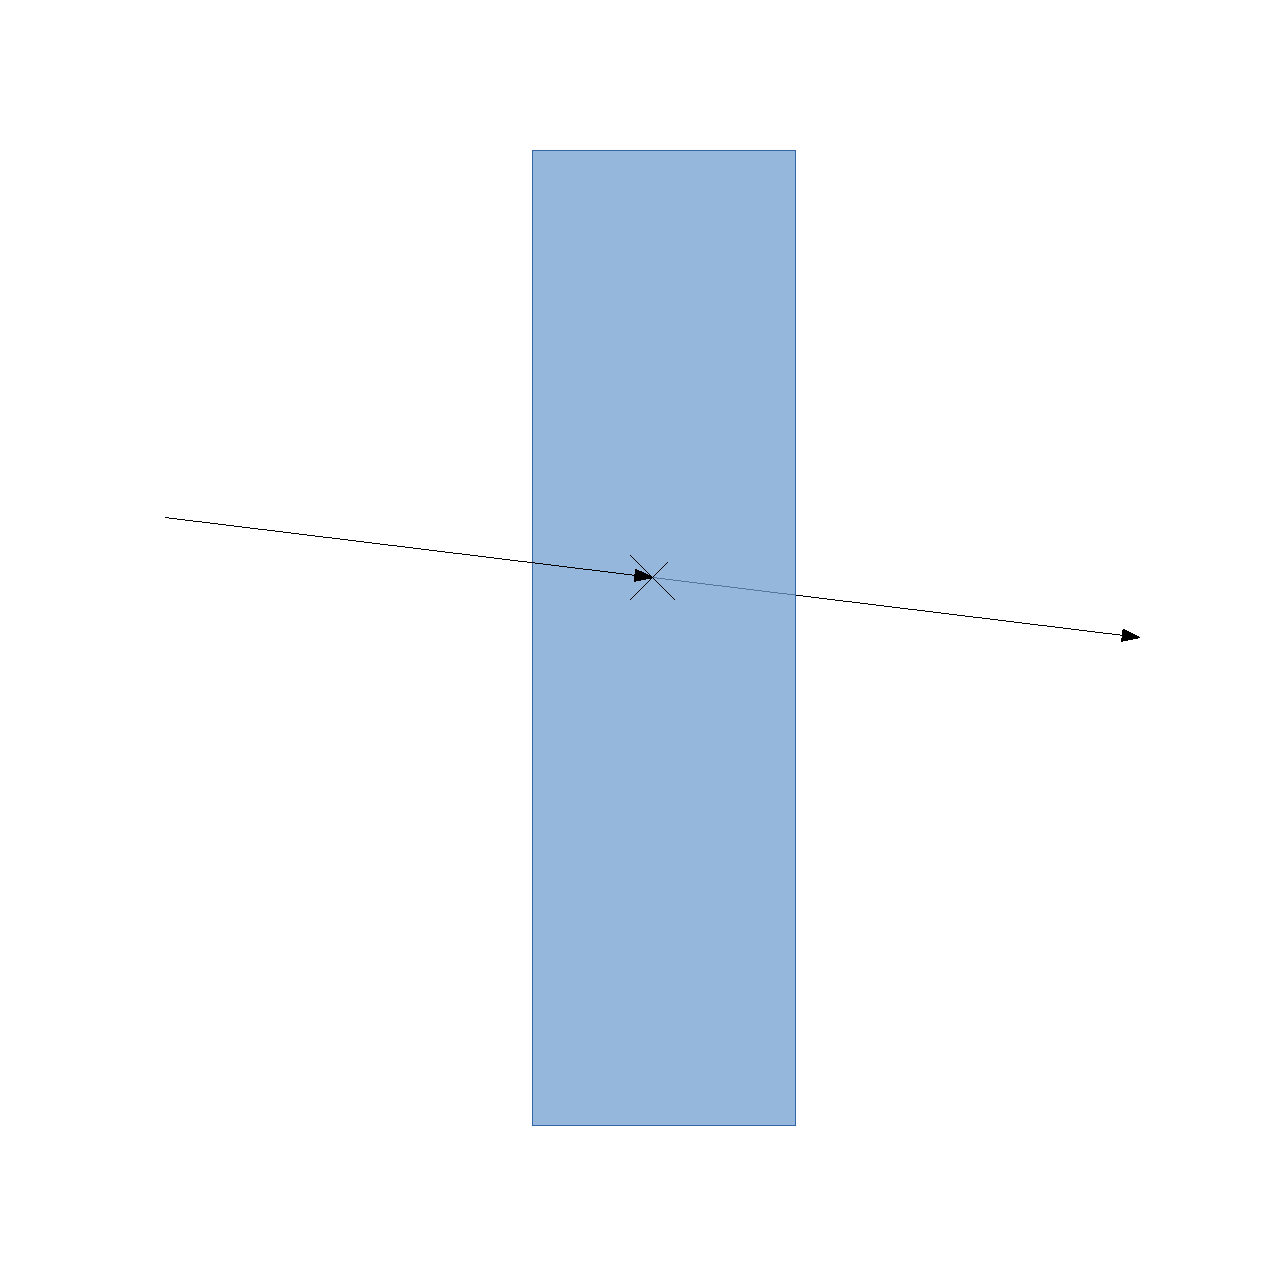
\includegraphics[angle=0,width=4in]{figures/theory/bz.pdf}
    \caption{Feynman diagram of two-fermion scattering.}
    \label{fig:feynmantwofermion}
  \end{figure}
  Figure~\ref{fig:feynmantwofermion} shows the Feynman diagram for two-fermion
  scattering. For a massive, vector-boson propagator the matrix element for
  this interaction is given by
  \begin{equation}\label{eq:genmatel}
    \mathcal{M} = \mel{f}{S}{i} = \mel{k'}{J^{\mu}(0)}{k} \frac{i}{q^2 - M_V^2}(-g_{\mu\nu} 
            + q_{\mu}q_{\nu}/M_V^2) \mel{p'}{J^{\mu}(0)}{p} \,,
  \end{equation}
  where $k$ and $k'$ initial and final four-momenta of the first fermion
  ($f_1$), $p$ and $p'$ are the initial and final four-momenta of the second
  fermion ($f_2$), $q$ is the four-momenta carried by the vector-boson
  propagator, and $M_V$ is the mass of the propagator, and $J^{\mu}$ is the
  probability current operator.


%%%%%%%%%%%%%%%%%%%%%%%%%%%%%%%%%%%%%%%%%%%%%%%%%%%%%%%%%%%
% Electroweak Interactions
%%%%%%%%%%%%%%%%%%%%%%%%%%%%%%%%%%%%%%%%%%%%%%%%%%%%%%%%%%%
\subsection{Electroweak interactions}

  The charged current, $j^{\mu}_{CC}$, which corresponds to the exchange of a
  $W^{\pm}$ boson, and the neutral current, $j^{\mu}_{NC}$, which corresponds
  to the exchange of the $Z^0$ boson are given by
  \begin{align}\label{eq:ccurrent}
      j^{\mu}_{CC} &= \sum_f \bar{\psi}_f \gamma^{\mu} (1-\gamma_5) \frac{1}{2}(\tau_1 + i\tau_2) \psi_f \\
        \label{eq:ncurrent}
      j^{\mu}_{NC} &= \sum_f \bar{\psi}_f \gamma^{\mu} (1-\gamma_5) \frac{1}{2}(\tau_3) \psi_f 
       - 2\sin^2(\theta_W) j^{\mu}_{em}
  \end{align}
  where $j^{\mu}_{em}$ is the electromagnetic current, $\psi_{f}$ are the weak
  isospin doublets, and $\tau_i$ are the Pauli matrices
  \begin{equation}
      \tau_1 = 
      \begin{pmatrix}
        0 & 1 \\
        1 & 0
      \end{pmatrix} \,,
      \hspace{5mm}
      \tau_2 = 
      \begin{pmatrix}
        0 & -i \\
        i & 0
      \end{pmatrix} \,,
      \hspace{5mm}
      \tau_3 = 
      \begin{pmatrix}
        1 & 0 \\
        0 & -1
      \end{pmatrix} \,.
  \end{equation}
  The lepton weak isospin doublets are
  \begin{equation}
    \psi_{e} = 
    \begin{pmatrix}
        \hat{\nu}_{e} \\
        \hat{e}^-
    \end{pmatrix} \,,
      \hspace{5mm}
    \psi_{\mu} = 
    \begin{pmatrix}
        \hat{\nu}_{\mu} \\
        \hat{\mu}^-
    \end{pmatrix} \,,
      \hspace{5mm}
    \psi_{\tau} = 
    \begin{pmatrix}
        \hat{\nu}_{\tau} \\
        \hat{\tau}^-
    \end{pmatrix} \,,
  \end{equation}
  and the quark weak isospin doublets are
  \begin{equation}
    \psi_{1} = 
    \begin{pmatrix}
        \hat{u} \\
        \hat{d'}
    \end{pmatrix} \,,
      \hspace{5mm}
    \psi_{2} = 
    \begin{pmatrix}
        \hat{c} \\
        \hat{s'}
    \end{pmatrix} \,,
      \hspace{5mm}
    \psi_{3} = 
    \begin{pmatrix}
        \hat{t} \\
        \hat{b'}
    \end{pmatrix} \,,
  \end{equation}
  where $d'$, $s'$, and $b'$ represent the ``mixed" states
  \begin{equation}
      \begin{pmatrix}
        \hat{d}' \\
        \hat{s}' \\
        \hat{b}'
      \end{pmatrix}
      =
      \begin{pmatrix}
          V_{ud} & V_{us} & V_{ub} \\
          V_{cd} & V_{cs} & V_{cb} \\
          V_{td} & V_{ts} & V_{tb}
      \end{pmatrix}
      \begin{pmatrix}
        \hat{d} \\
        \hat{s} \\
        \hat{b}
      \end{pmatrix}
  \end{equation}
  where $V$ is the Cabibbo-Kobayashi-Maskawa matrix. These doublets contain the
  allowed weak transitions.

  \subsubsection{The charged current}
  The combination of Pauli matrices in the charged current
  \begin{equation}
      \frac{1}{2}\tau_+ = \frac{1}{2}(\tau_1 + \tau_2) \,,
  \end{equation}
  acts as an ``isospin raising matrix" and corresponds to the exchange of a
  $W^+$ boson.
  For the leptons, this gives
  \begin{equation}
    \begin{aligned}
      j^{\mu}_{CC}(\textrm{leptons}) &= \sum_{l=e,\mu,\tau}
      \begin{pmatrix}
          \bar{\hat{\nu}}_l \\
          \bar{\hat{l}}
      \end{pmatrix}
      \gamma^{\mu}(1-\gamma_5)\frac{1}{2}
      \begin{pmatrix}
        0 & 1 \\
        0 & 0
      \end{pmatrix}
      \begin{pmatrix}
        \hat{\nu}_l \\
          \hat{l}
      \end{pmatrix} \\
      &= \sum_{l=e,\mu,\tau} \bar{\hat{\nu}}_{l} \gamma^{\mu}(1-\gamma_5)\frac{1}{2}\, \hat{l} \,,
    \end{aligned}
  \end{equation}
  and, similarly, for the quarks we get
  \begin{equation}
      j^{\mu}_{CC}(\textrm{quarks}) =
       \bar{\hat{u}}\gamma^{\mu}(1-\gamma_5)\frac{1}{2}\,\hat{d}'
       +\bar{\hat{c}}\gamma^{\mu}(1-\gamma_5)\frac{1}{2}\,\hat{s}'
       +\bar{\hat{t}}\gamma^{\mu}(1-\gamma_5)\frac{1}{2}\,\hat{b}' \,,
  \end{equation}
  with the total charged current being $j^{\mu}_{CC} =
  j^{\mu}_{CC}(\textrm{leptons}) + j^{\mu}_{CC}(\textrm{quarks})$.

  \subsubsection{The neutral current}
  In neutral current scattering, $\frac{1}{2}\tau_3$ gives the weak isospin
  which acts as a ``weak charge". The electromagnetic current is given by
  \begin{equation}
      j^{\mu}_{em} = \sum_f Q_f \bar{\hat{f}} \gamma^{\mu} \hat{f}
  \end{equation}
  where $f$ is the fermions, and $Q_f$ is the electric charge of $f$.
  So, the total neutral current is
  \begin{equation}
    \begin{aligned}
        j^{\mu}_{NC} &= \sum_{l=e,\mu,\tau} \left(\bar{\hat{\nu}}_{l}
        \gamma^{\mu}(1-\gamma_5) \frac{1}{2}\, \hat{\nu}_{l} - \bar{\hat{l}}
        \gamma^{\mu}(1-\gamma_5) \frac{1}{2}\, \hat{l} 
        +\sin^2\theta_W \bar{\hat{l}}\gamma^{\mu}\hat{l} \right) \\
        &+ \sum_{q=u,c,t} \left(\bar{\hat{q}} \gamma^{\mu}(1-\gamma_5)\frac{1}{2}\hat{q} 
        - \sin^2\theta_W \frac{2}{3} \bar{\hat{q}}\gamma^{\mu}\hat{q} \right) \\
        &+ \sum_{q=d,s,b} \left(- \bar{\hat{q}} \gamma^{\mu}(1-\gamma_5)\frac{1}{2}\hat{q} 
        + \sin^2\theta_W \frac{1}{3} \bar{\hat{q}}\gamma^{\mu}\hat{q} \right) \,.
     \end{aligned}
  \end{equation}
 
  \subsubsection{V$-$A structure}

  We can separate the currents into their vector and pseudovector, or axial
  vector, components. The terms that contain just $\gamma^{\mu}$ behave like
  vectors under a parity transformation
  \begin{equation}
    \hat{\textrm{\textbf{P}}}\hat{\psi}(\textbf{x},t)\hat{\textrm{\textbf{P}}}^{-1} \, 
      \gamma^{\mu} \, \hat{\textrm{\textbf{P}}}\hat{\psi(\textbf{x},t)}\hat{\textrm{\textbf{P}}}^{-1} 
      = - \hat{\textrm{\textbf{P}}}\hat{\psi}(-\textbf{x},t)\hat{\textrm{\textbf{P}}}^{-1} \, 
      \gamma^{\mu} \, \hat{\textrm{\textbf{P}}}\hat{\psi(-\textbf{x},t)}\hat{\textrm{\textbf{P}}}^{-1}
  \end{equation}
  where $\hat{\textrm{\textbf{P}}}$ is the parity operator
  \begin{equation}
    \textrm{\textbf{P}}: \textbf{x} \rightarrow -\textbf{x}, t \rightarrow t \,.
  \end{equation}
  The terms that contain $\gamma^{\mu}\gamma_{5}$ behave like axial vectors
  under a parity transformation
  \begin{equation}
    \hat{\textrm{\textbf{P}}}\hat{\psi}(\textbf{x},t)\hat{\textrm{\textbf{P}}}^{-1} \, 
      \gamma^{\mu}\gamma_5 \, \hat{\textrm{\textbf{P}}}\hat{\psi(\textbf{x},t)}\hat{\textrm{\textbf{P}}}^{-1} 
      = + \hat{\textrm{\textbf{P}}}\hat{\psi}(-\textbf{x},t)\hat{\textrm{\textbf{P}}}^{-1} \, 
      \gamma^{\mu}\gamma_5 \, \hat{\textrm{\textbf{P}}}\hat{\psi(-\textbf{x},t)}\hat{\textrm{\textbf{P}}}^{-1}
      \,.
  \end{equation}
  The charged current is simple
  \begin{equation}
    \begin{aligned}
    j^{\mu}_{CC} = \frac{g}{\sqrt{2}}\Bigg[&\sum_{l=e,\mu,\tau} \bar{\hat{\nu}}_l (\gamma^{\mu} 
          - \gamma^{\mu}\gamma_5)\frac{1}{2}\,\hat{l} \\
      &+ \bar{\hat{u}}(\gamma^{\mu} - \gamma^{\mu}\gamma_5)\frac{1}{2}\, \hat{d}'
      + \bar{\hat{c}}(\gamma^{\mu} - \gamma^{\mu}\gamma_5)\frac{1}{2}\, \hat{s}'
      + \bar{\hat{t}}(\gamma^{\mu} - \gamma^{\mu}\gamma_5)\frac{1}{2}\, \hat{b}' \Bigg] \,,
    \end{aligned}
  \end{equation}
  and the neutral current becomes
  \begin{equation}
    \begin{aligned}
        j^{\mu}_{NC} = \frac{g}{2\cos\theta_W} \Bigg[&\sum_{l=e,\mu,\tau} 
        \left(\bar{\hat{\nu}}_{l}(g_V^{l} \gamma^{\mu}- g_A^{l} \gamma^{\mu}\gamma_5) \hat{\nu}_{l} 
         + \bar{\hat{l}}(g_V^{l} \gamma^{\mu}- g_A^{l} \gamma^{\mu}\gamma_5)\, \hat{l} \right) \\
        &+ \sum_{q=u,d,c,s,t,b} 
         \left(- \bar{\hat{q}} (g_V^{q} \gamma^{\mu}-g_A^{q} \gamma^{\mu}\gamma_5)\hat{q} \right)\Bigg] \,.
     \end{aligned}
  \end{equation}
  where 
  \begin{equation}
    g_V^{f} = \frac{1}{2}\tau_3^{f} - 2\sin^2\theta_W Q_f \,,
    \hspace{3mm}
    g_A^{f} = \frac{1}{2}\tau_3^{f} \,.
  \end{equation}

%%%%%%%%%%%%%%%%%%%%%%%%%%%%%%%%%%%%%%%%%%%%%%%%%%%%%%%%%%%
% Electroweak Scattering Matrix Elements
%%%%%%%%%%%%%%%%%%%%%%%%%%%%%%%%%%%%%%%%%%%%%%%%%%%%%%%%%%%
\subsection{Electroweak Scattering Matrix Elements}

  \begin{figure}[h]
    \centering
    \begin{subfigure}{2.5in}
      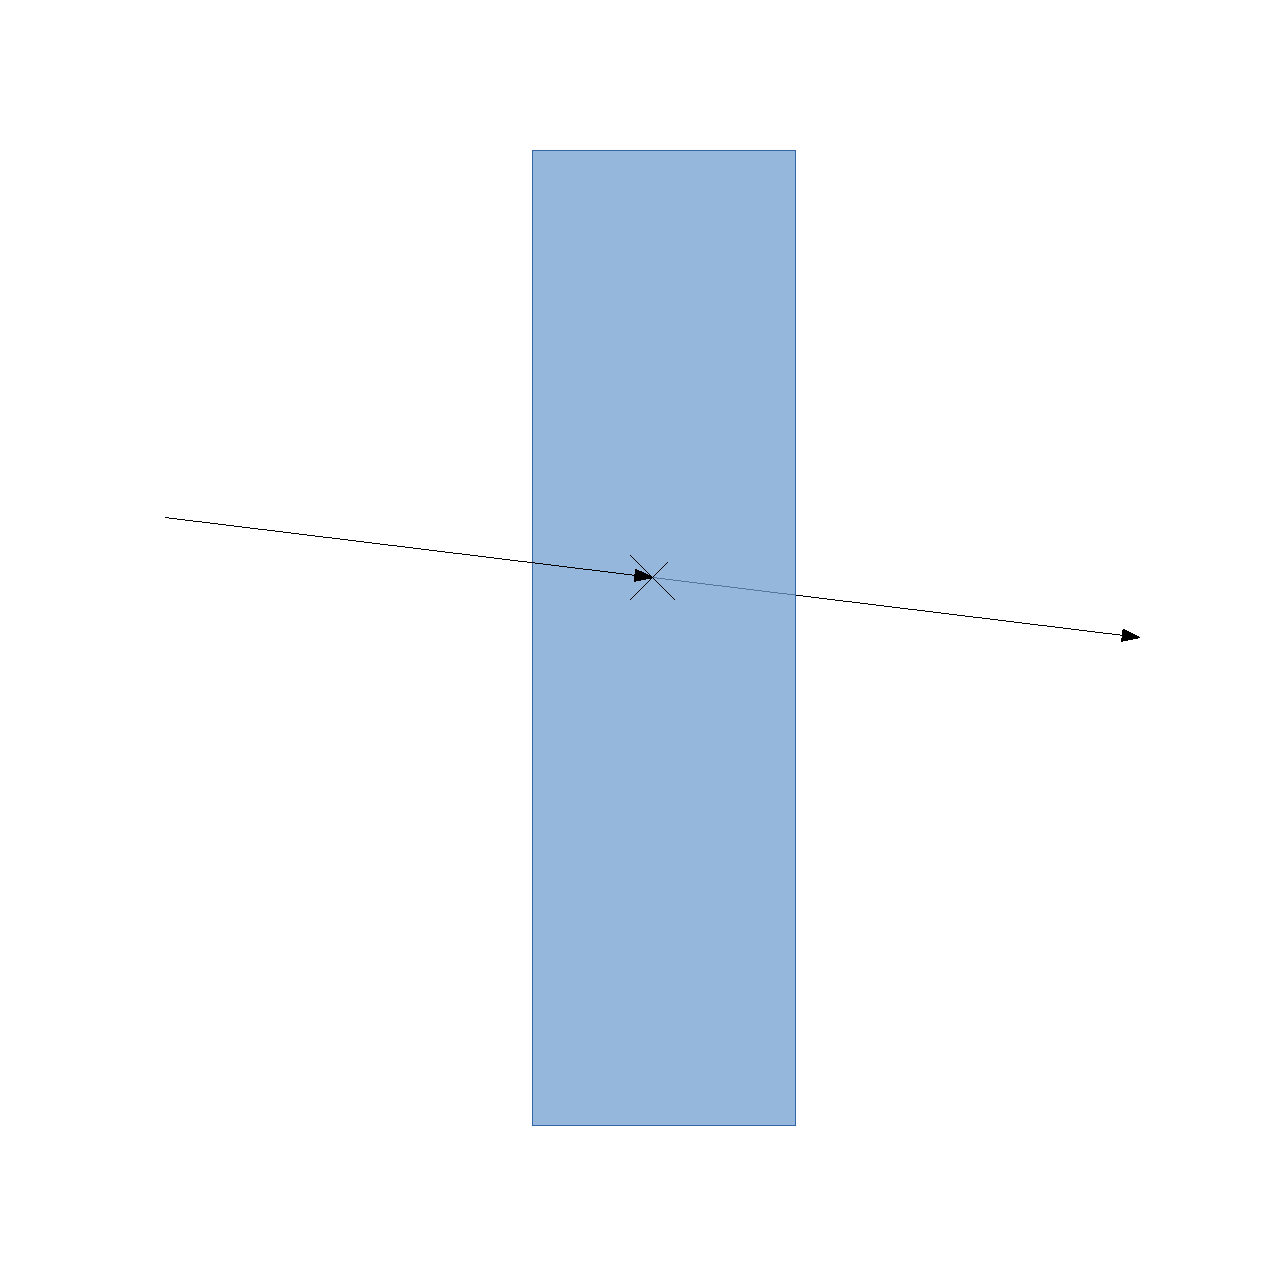
\includegraphics[angle=0,width=2.5in]{figures/theory/bz.pdf}
      \caption{Feynman diagram of neutral-current elastic lepton-nucleon
      scattering.}
      \label{fig:ncefeynman}
    \end{subfigure}
    \hspace{2pt}
    \begin{subfigure}{2.5in}
      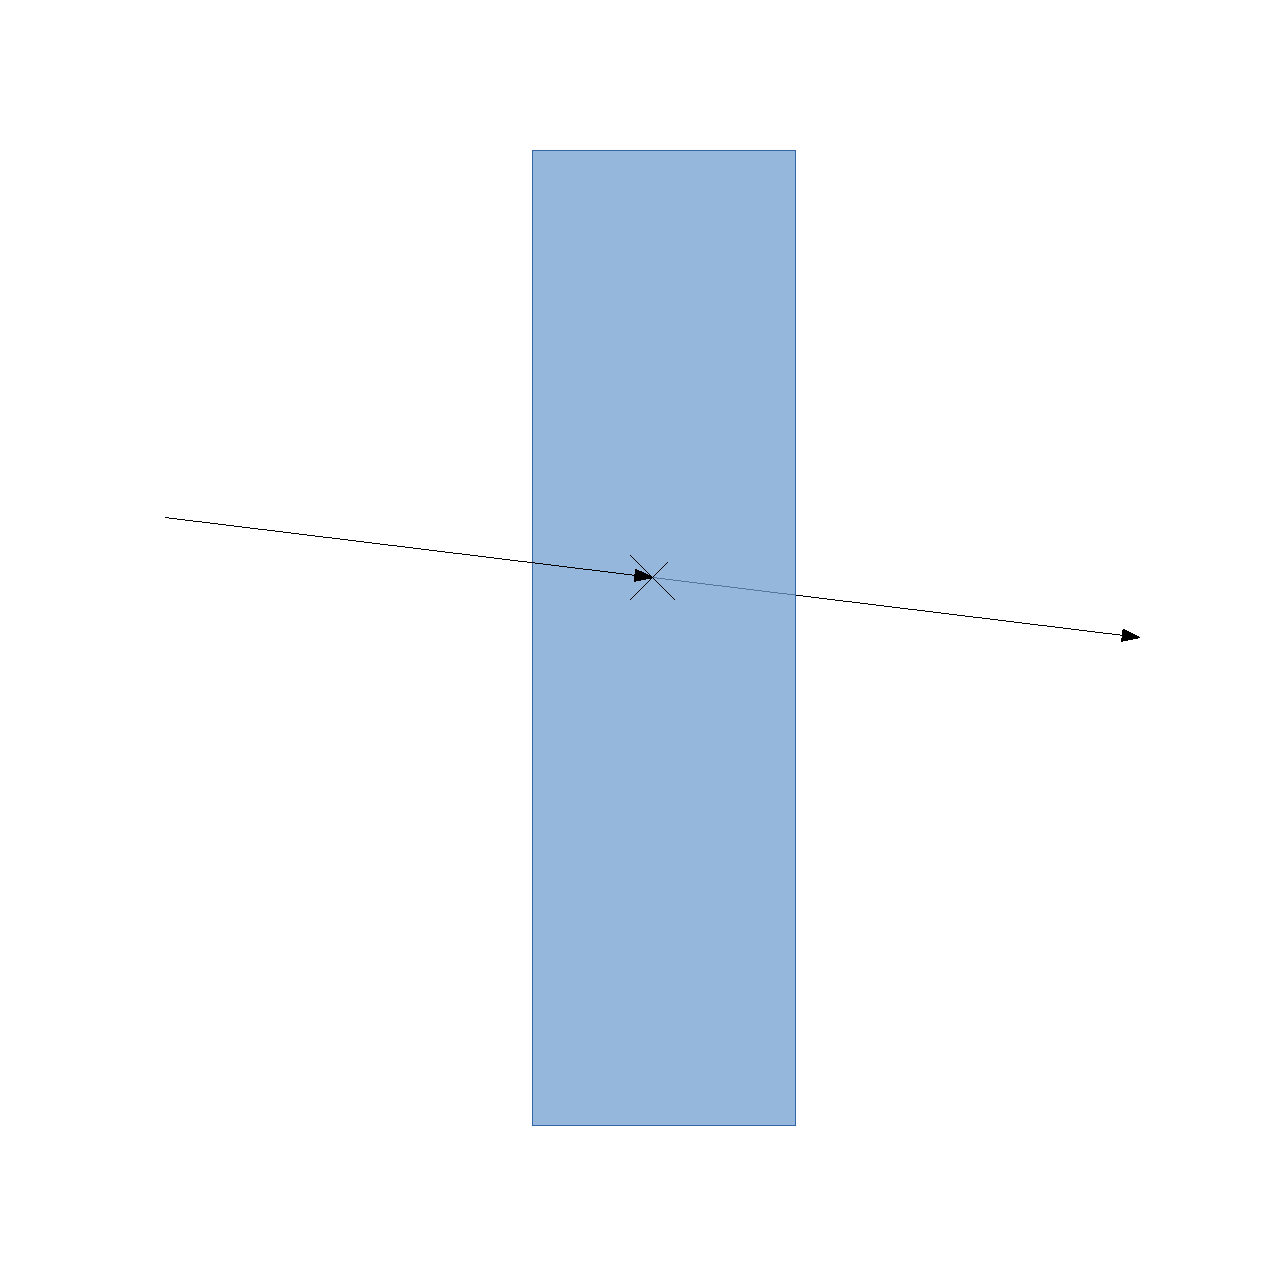
\includegraphics[angle=0,width=2.5in]{figures/theory/bz.pdf}
      \caption{Feynman diagram of charged-current elastic lepton-nucleon
      scattering.}
      \label{fig:ccqefeynman}
    \end{subfigure}
  \end{figure}

  To calculate the charged-current neutrino-nucleon scattering matrix element,
  as shown in Fig.~\ref{fig:ccqefeynman}, we need to determine the lepton CC
  matrix element, $_{l}\mel{k'}{J^{\mu}_{CC}(0)}{k}_{\nu_l}$, and the nucleon
  CC matrix element, $_{\textrm{p}}\mel{p'}{J^{\mu}_{CC}(0)}{p}_{\textrm{n}}$,
  and for neutral-current, as shown in Fig.~\ref{fig:ncefeynman}, we need the
  lepton NC matrix element, $_{\nu_l}\mel{k'}{J^{\mu}_{NC}(0)}{k}_{\nu_l}$, and
  the nucleon NC matrix element,
  $_{\textrm{p}}\mel{p'}{J^{\mu}_{NC}(0)}{p}_{\textrm{p}}$. Leptons are
  point-like particles, so their matrix elements are straight-forward
  \begin{equation}
    \begin{aligned}
      _l\mel{k'}{J^{\mu}_{CC}(0)}{k}_{\nu_l}
        &= -i\frac{G_F}{\sqrt{2}}\bar{u}(k')(\gamma^{\mu} - \gamma^{\mu}\gamma_5)u(k) \,, \\
        _{\nu_l}\mel{k'}{J^{\mu}_{NC}(0)}{k}_{\nu_l}
        &= -\frac{G_F}{\sqrt{2}}\bar{u}(k')(\gamma^{\mu} - \gamma^{\mu}\gamma_5)u(k) \,.
    \end{aligned}
  \end{equation}

  \subsubsection{Nucleon matrix elements}
  Since nucleons have a finite structure, the nucleon matrix elements have a
  more complicated form. The current is corrected by form factors which encode
  the longitudinal nucleon structure.

  If we define the vector and axial parts of the nucleon currents by
  \begin{equation}
    \begin{aligned}
    v^{\mu}_i &= \bar{\hat{\psi}}_f\, \gamma^{\mu}\frac{1}{2}\tau_i\, \hat{\psi}_f \,, \\
    a^{\mu}_i &= \bar{\hat{\psi}}_f\, \gamma^{\mu}\gamma_5\frac{1}{2}\tau_i\, \hat{\psi}_f \,,
    \end{aligned}
  \end{equation}
  where $\hat{\psi}$ are the quark doublets and $\tau_i$ are the Pauli matrices
  still, then the nucleon charged and neutral current become
  \begin{equation}
    \begin{aligned}
      j^{\mu}_{CC} &= v^{\mu}_+ - a^{\mu}_+ \,, \\
      j^{\mu}_{NC} &= v^{\mu}_3 - a^{\mu}_3 - 2\sin^2\theta_W j^{\mu}_{em;q} \,,
    \end{aligned}
  \end{equation}
  where $v^{\mu}_+ = v^{\mu}_1 + iv^{\mu}_2$ and $a^{\mu}_+ = a^{\mu}_1 +
  ia^{\mu}_2$. The nucleon matrix elements become
  \begin{equation}
    \begin{aligned}
      _{\textrm{p}}\mel{p'}{J^{\mu}_{CC}}{p}_{\textrm{n}}
          &= _{\textrm{p}}\mel{p'}{V^{\mu}_{+}}{p}_{\textrm{n}}
            - _{\textrm{p}}\mel{p'}{A^{\mu}_{+}}{p}_{\textrm{n}} \,, \\
      _{\textrm{p}}\mel{p'}{J^{\mu}_{NC}}{p}_{\textrm{p}}
          &= _{\textrm{p}}\mel{p'}{V^{\mu}_{3}}{p}_{\textrm{p}} 
            - _{\textrm{p}}\mel{p'}{A^{\mu}_{3}}{p}_{\textrm{p}} 
            - _{\textrm{p}}\mel{p'}{J^{\mu}_{em}}{p}_{\textrm{p}} \,,
    \end{aligned}
  \end{equation}
  where $J^{\mu}$, $V^{\mu}$, and $A^{\mu}$ are current operators.

  \subsubsection{Electromagnetic Scattering}

  It is easiest to first find an equation for $j^{\mu}_{em;q}$ in terms of the
  electric and magnetic form factors. The nucleon electromagnetic current
  should have the same vector form as the electromagnetic current for
  point-like particles. The available physical variables to construct the
  nucleon EM current are $p$, $p'$, $\gamma^{\mu}$. The most general form is
  \begin{equation}
    \Gamma^{\mu} = \gamma^{\mu}\cdot A + (p'^{\mu} + p^{\mu})\cdot B + (p'^{\mu} - p^{\mu})\cdot C \,,
  \end{equation}
  where $\Gamma^{\mu}$ is given by the equation
  $_{\textrm{p}}\mel{p'}{J^{\mu}_{em}(0)}{p}_{\textrm{p}} =
  \bar{u}(p')\Gamma^{\mu}u(p)$, and $A$, $B$, and $C$ are arbitrary form
  factors.  $\Gamma^{\mu}$ if constrained further by the Ward identity,
  $q_{\mu}\Gamma^{\mu} = 0$, which guarantees current conservation. The
  $\gamma^{\mu}$ and $(p'^{\mu} + p^{\mu})$ terms in $q_{\mu}\Gamma^{\mu}$ go
  to zero, but the $(p'^{\mu} - p^{\mu})$ term does not, so $C=0$. Using the
  Gordon identity~\cite{Gordon}, the general form for the nucleon EM current
  matrix element is
  \begin{equation}\label{eq:FFem}
    _{\textrm{p}}\mel{p'}{J^{\mu}_{em}(0)}{p}_{\textrm{p}} =
      \bar{u}(p')\left[ \gamma^{\mu}F_1(Q^2) + \frac{i\sigma^{\mu\nu}q_{\mu}}{2M}F_2(Q^2)  \right]u(p) \,.
  \end{equation}
  The form factors $F_1$ and $F_2$ are the Dirac and Pauli form factors,
  respectively, and they are functions of $Q^2 = -q^2$. They can be transformed
  into the Sachs form factors, $G_E$ and $G_M$ by the relationships
  \begin{equation}
    G_E(Q^2) = F_1(Q^2) - \frac{Q^2}{4M^2}F_2(Q^2)\,, \hspace{5mm} G_M(Q^2) = F_1(Q^2) + F_2(Q^2) \,,
  \end{equation}
  where $Q^2 = -q^2$.  The electric form factor, $G_E$ encodes the longitudinal
  electric charge structure of the nucleon and the magnetic form factor, $G_M$,
  encodes the longitudinal magnetic structure. At the limit when $Q^2$ goes to
  zero, the Sachs form factors become the net charge and magnetic moment of the
  nucleon.
  \begin{equation}
    \begin{aligned}
      G_{E;p}(Q^2=0) = 1 \,,& \hspace{5mm} G_{M;p}(Q^2=0) = \mu_p \,, \\
      G_{E;n}(Q^2=0) = 0 \,,& \hspace{5mm} G_{M;n}(Q^2=0) = \mu_n \,,
    \end{aligned}
  \end{equation}
  where $\mu_p$ and $\mu_n$ are the proton and neutron magnetic moments.
 
  \subsubsection{Vector current}

    The quark part of the electromagnetic current, $j^{\mu}_{em;q}$, can be
    written as
    \begin{equation}\label{eq:emcurrent30}
      \begin{aligned}
        j^{\mu}_{em;q} &= \bar{\hat{\psi}}_f \, Q_f \gamma^{\mu}\, \hat{\psi}_f \\
                       &= \bar{\hat{\psi}}_f \, (\tau_3 + \frac{1}{6})\gamma^{\mu} \, \hat{\psi}_f \\
                       &= v^{\mu}_3 + v^{\mu}_0 \,,
      \end{aligned}
    \end{equation}
    where $v^{\mu}_0 = \frac{1}{6}\bar{\hat{\psi}}_f \, \gamma^{\mu}
    \hat{\psi}_f$. Now we can write the nucleon electromagnetic current matrix
    element in terms of the vector and isoscalar parts
    \begin{equation}
      \begin{aligned}
        _{\textrm{p(n)}}\mel{p'}{J^{\mu}_{em}(0)}{p}_{\textrm{p(n)}} 
            &= _{\textrm{p(n)}}\mel{p'}{V^{\mu}_3(0) + V^{\mu}_0(0))}{p}_{\textrm{p(n)}} \\
            &= _{\textrm{p(n)}}\mel{p'}{V^{\mu}_3(0)}{p}_{\textrm{p(n)}} 
             + _{\textrm{p(n)}}\mel{p'}{V^{\mu}_0(0)}{p}_{\textrm{p(n)}} \,,
      \end{aligned}
    \end{equation}
    Since $V^{\mu}_3$ behaves like a vector under the charge symmetry operator and
    $V^{\mu}_0$ behaves as a scalar, the following equations are true
    \begin{equation}
      \begin{aligned}
        _{\textrm{p}}\mel{p'}{V^{\mu}_3(0)}{p}_{\textrm{p}} 
          &= - _{\textrm{n}}\mel{p'}{V^{\mu}_3(0)}{p}_{\textrm{n}} \,, \\
        _{\textrm{p}}\mel{p'}{V^{\mu}_0(0)}{p}_{\textrm{p}} 
          &= + _{\textrm{n}}\mel{p'}{V^{\mu}_0(0)}{p}_{\textrm{n}} \,. \\
      \end{aligned}
    \end{equation}
    Then
    \begin{align}\label{eq:V3em}
      _{\textrm{p}}\mel{p'}{V^{\mu}_3(0)}{p}_{\textrm{p}} 
        &= \frac{1}{2} \left[_{\textrm{p}}\mel{p'}{J^{\mu}_{em}(0)}{p}_{\textrm{p}} 
         - _{\textrm{n}}\mel{p'}{J^{\mu}_{em}(0)}{p}_{\textrm{n}} \right] \,, \\
      _{\textrm{p}}\mel{p'}{V^{\mu}_0(0)}{p}_{\textrm{p}} 
        &= \frac{1}{2} \left[_{\textrm{p}}\mel{p'}{J^{\mu}_{em}(0)}{p}_{\textrm{p}} 
         + _{\textrm{n}}\mel{p'}{J^{\mu}_{em}(0)}{p}_{\textrm{n}} \right] \,.
    \end{align}
    Combining equations~\ref{eq:FFem}~and~\ref{eq:V3em} gives
    \begin{equation}
      _{\textrm{p}}\mel{p'}{V^{\mu}_3(0)}{p}_{\textrm{p}} 
        = \bar{u}(p') \left[\gamma^{\mu}F_1^V(Q^2) 
          + \frac{i\sigma^{\mu\nu}q_{\mu}}{2M}F_2^V(Q^2)\right] u(p) \,,
    \end{equation}
    where the vector form factors, $F_1^V$ and $F_2^V$ are defined as
    \begin{equation}
      \begin{aligned}
        F_1^V(Q^2) &= \frac{1}{2}\left( F_{1,\textrm{p}}(Q^2) - F_{1,\textrm{n}}(Q^2)\right) \,, \\
        F_2^V(Q^2) &= \frac{1}{2}\left( F_{2,\textrm{p}}(Q^2) - F_{2,\textrm{n}}(Q^2)\right) \,.
      \end{aligned}
    \end{equation}

    The isoscalar nucleon matrix element is then
    \begin{equation}
      {\mel{p'}{V^{\mu}_0(0)}{p}}
      = \bar{u}(p')\left[\gamma^{\mu}\frac{1}{2}\left(F_{1,p}(Q^2) + F_{1,n}(Q^2)\right) 
        + \frac{i\sigma^{\mu\nu}q_{\mu}}{2M}\frac{1}{2}\left(F_{2,p}(Q^2) + F_{2,n}(Q^2)\right)\right]u(p)
    \end{equation}
 
    Under the conserved vector current (CVC) hypothesis the ``raising" and
    ``lowering" vector currents, $v^{\mu}_{\pm}$, in the charged current
    interactions are the same as the vector part of the electromagnetic current,
    $v^{\mu}_{3}$.

  \subsubsection{Axial current}

    The axial current nucleon matrix elements can also be parameterized in
    terms of form factors. Starting with the charged axial current, the most
    general form contains an axial, a pseudoscalar, and a tensor term,
    \begin{equation}
      _{\textrm{p}}\mel{p'}{A^{\mu}_+(0)}{p}_{\textrm{n}} 
        = \bar{u}(p') \left[\gamma^{\mu}\gamma^{5} G_A(Q^2) 
          + \frac{q^{\mu}\gamma^{5}}{2M}G_P^{CC}(Q^2) 
          + \frac{\eta^{\mu}\gamma^{5}}{2M}G_T^{CC}(Q^2)\right] u(p) \,,
    \end{equation}
    where $G_A$, $G_P^{CC}$, and $G_T^{CC}$ are form factors and $\eta^{\mu}$
    is the metric tensor. From isospin symmetry, we have
    \begin{equation}
      _{\textrm{p}}\mel{p'}{A^{\mu}_+(0)}{p}_{\textrm{n}} 
      = _{\textrm{n}}\mel{p'}{A^{\mu}_-(0)}{p}_{\textrm{p}} 
      \equiv _{\textrm{p}}\mel{p}{A^{\mu}_+(0)}{p'}_{\textrm{n}}^* \,,
    \end{equation}
    which implies that $G_T^{CC}(Q^2) = 0$. In quasi-elastic scattering the
    pseudoscalar term containing $G_P^{CC}(Q^2)$ is proportional to the lepton
    mass, and is often ignored. The charged current axial matrix element is then just
    \begin{equation}
      _{\textrm{p}}\mel{p'}{A^{\mu}_+(0)}{p}_{\textrm{n}} 
        = \bar{u}(p') \,\gamma^{\mu}\gamma^{5} G_A(Q^2)\, u(p) \,.
    \end{equation}
    The form factor $G_A$ encodes the longitudinal spin structure of the
    nucleon due to the spin of the up and down quarks and is referred to as the
    charged current axial form factor, or just the axial form factor.

    The most general form for the neutral axial current nucleon matrix element
    is similarly
    \begin{equation}
      _{\textrm{p}}\mel{p'}{A^{\mu}_3(0)}{p}_{\textrm{n}} 
        = \bar{u}(p') \left[\gamma^{\mu}\gamma^{5} G_A^{NC}(Q^2) 
          + \frac{q^{\mu}\gamma^{5}}{2M}G_P^{NC}(Q^2) 
          + \frac{\eta^{\mu}\gamma^{5}}{2M}G_T^{NC}(Q^2)\right] u(p) \,.
    \end{equation}
    Just as in the charged-current case, tensor part is zero, $G_T^{NC}(Q^2) =
    0$, and we can again neglect $G_P^{NC}$ which is proportional to the lepton
    mass. The neutral axial current matrix element is
    \begin{equation}
      _{\textrm{p}}\mel{p'}{A^{\mu}_3(0)}{p}_{\textrm{n}} 
        = \bar{u}(p') \,\gamma^{\mu}\gamma^{5} G_A^{NC}(Q^2)\, u(p) \,.
    \end{equation}
    which can be related to the charged current axial form factor through
    isospin symmetry.  The relationship is between the neutral and charged
    axial current operators is
    \begin{equation}
      [I^k,A_j^{\mu}] = i\epsilon^{kjl}A^{\mu}_l \,,
    \end{equation}
    where $I^k$ is the total isospin operator, and $\epsilon^{kjl}$ is the
    antisymmetric tensor. From this relationship, we get
    \begin{equation}
      _{\textrm{p}}\mel{p'}{A^{\mu}_3(0)}{p}_{\textrm{p}}
       = \frac{1}{2}_{\textrm{p}}\mel{p'}{A^{\mu}_+(0)}{p}_{\textrm{n}}\,,
    \end{equation}
    which implies
    \begin{equation}
      G_A^{NC}(Q^2) = \frac{1}{2}G_A(Q^2) \,,
    \end{equation}
    assuming only the contributions from up and down quarks.

%%%%%%%%%%%%%%%%%%%%%%%%%%%%%%%%%%%%%%%%%%%%%%%%%%%%%%%%%%%
% Strangeness in the Nucleon
%%%%%%%%%%%%%%%%%%%%%%%%%%%%%%%%%%%%%%%%%%%%%%%%%%%%%%%%%%%
\subsection{Strangeness in the nucleon} \label{sec:strangeness}

  If contributions to the nucleon from quarks heavier than the strange are
  neglected, the quark part of the charged and neutral currents can be
  separated between the light quarks and the strange quark,
  \begin{equation}\label{eq:chargedcurrent}
    \begin{aligned}
    j^{\mu}_{CC}(\textrm{quarks}) &= \bar{\hat{u}}(\gamma^{\mu} 
                - \gamma^{\mu}\gamma_5)\frac{1}{2}\tau_{\pm}\hat{u}
                - \bar{\hat{d}}(\gamma^{\mu} - \gamma^{\mu}\gamma_5)\frac{1}{2}\tau_{\pm}\hat{d} \\
                 &\equiv \bar{\hat{N}}(\gamma^{\mu} 
                - \gamma^{\mu}\gamma_5)\frac{1}{2}\tau_{\pm}\hat{N} \,,
    \end{aligned}
  \end{equation}
  \begin{equation}\label{eq:neutralcurrent}
    \begin{aligned}
    j^{\mu}_{NC}(\textrm{quarks}) = \bar{\hat{N}}(\gamma^{\mu} 
                - \gamma^{\mu}\gamma_5)\frac{1}{2}\tau_3\hat{N} 
                &- \bar{\hat{s}}(\gamma^{\mu} - \gamma^{\mu}\gamma_5)\frac{1}{2}\tau_3\hat{s}  \\
                  &- 2\sin^2\theta_W j^{\mu}_{em;q} \,.
    \end{aligned}
  \end{equation}

  \subsubsection{Strange currents}
    If we redefine the neutral vector currents as
    \begin{equation}\label{eq:updowncurrents}
      \begin{aligned}
        v^{\mu}_3 &\equiv \bar{\hat{N}} \gamma^{\mu}\frac{1}{2}\tau_3 \hat{N} \\
        a^{\mu}_3 &\equiv \bar{\hat{N}} \gamma^{\mu}\gamma_5\frac{1}{2}\tau_3 \hat{N} \,,
      \end{aligned}
    \end{equation}
    and define the strange part of the currents as
    \begin{equation}\label{eq:strangecurrents}
      \begin{aligned}
        v^{\mu}_s &\equiv \bar{\hat{s}} \gamma^{\mu} \hat{s} \\
        a^{\mu}_s &\equiv \bar{\hat{s}} \gamma^{\mu}\gamma_5 \hat{s} \,,
      \end{aligned}
    \end{equation}
    we can rewrite combine
    Eqs.~\ref{eq:chargedcurrent},~\ref{eq:neutralcurrent},~\ref{eq:updowncurrents},~and~\ref{eq:strangecurrents}
    to get
    \begin{align}
      j^{\mu}_{CC}(\textrm{quarks}) &= (v^{\mu}_3 - a^{\mu}_3) \,, \\
      j^{\mu}_{NC}(\textrm{quarks}) &= (v^{\mu}_3 - a^{\mu}_3) 
        - \frac{1}{2}(v^{\mu}_s - a^{\mu}_s) - 2\sin^2\theta_W j^{\mu}_{em;q} \,.
    \end{align}
    
    The quark part of the electromagnetic current can also be separated into
    light and heavy quark components. Separating the vector and isoscalar terms
    from Eq.~\ref{eq:emcurrent30}, into quark components gives
    \begin{equation}
      j^{\mu}_{em;q} = (v^{\mu}_3 + v^{\mu}_0) - \frac{1}{2}(v^{\mu}_s + v^{\mu}_{0s}) \,,
    \end{equation}
    where $v^{\mu}_3$ and $v^{\mu}_s$ are as defined in
    Eqs.~\ref{eq:updowncurrents}~and~\ref{eq:strangecurrents}, and $v^{\mu}_0$
    and $v^{\mu}_s0$ are defined as
    \begin{equation}
      \begin{aligned}
        v^{\mu}_0 &\equiv \frac{1}{6}\bar{\hat{N}}\gamma^{\mu}\hat{N} \,, \\
        v^{\mu}_{0s} &\equiv -\frac{1}{3}\bar{\hat{s}}\gamma^{\mu}\hat{s} \,.
      \end{aligned}
    \end{equation}
    The quark part of the neutral current becomes
    \begin{equation}
      j^{\mu}_{NC}(\textrm{quarks}) = (1-2\sin^2\theta_W)(v^{\mu}_3 - \frac{1}{2}v^{\mu}_s)
                                    - (a^{\mu}_3 - \frac{1}{2}a^{\mu}_s)
                                    - 2\sin^2\theta_W(v^{\mu}_0 - \frac{1}{2}v^{\mu}_{0s}) \,.
    \end{equation}

  \subsubsection{Strange nucleon matrix elements}

  The single-nucleon matrix elements for the charged current becomes
  \begin{equation}
     _{\textrm{p}}\mel{p'}{J^{\mu}_{CC}(0)}{p}_{\textrm{n}} 
       = _{\textrm{p}}\mel{p'}{V^{\mu}_3(0)}{p}_{\textrm{n}}
       - _{\textrm{p}}\mel{p'}{A^{\mu}_3(0)}{p}_{\textrm{n}} \,.
  \end{equation}
  In terms of the vector and axial form factors, the matrix element is
  \begin{equation}
     _{\textrm{p}}\mel{p'}{J^{\mu}_{CC}(0)}{p}_{\textrm{n}}
       = \bar{u}(p')\left[\gamma^{\mu} F_1^V(Q^2)
          + \frac{i\sigma^{\mu\nu}q_{\mu}}{2M} F_2^V(Q^2)
          - \gamma^{\mu}\gamma_5G_A(Q^2) \right] u(p) \,.
  \end{equation}
  The single-nucleon matrix elements for the neutral current becomes
  \begin{equation}
    \begin{aligned}
      _{\textrm{p}}\mel{p'}{J^{\mu}_{NC}(0)}{p}_{\textrm{p}} 
       = (1-2\sin^2\theta_w)&(_{\textrm{p}}\mel{p'}{V^{\mu}_3(0)}{p}_{\textrm{p}}
        - _{\textrm{p}}\mel{p}{\frac{1}{2}V^{\mu}_s(0)}{p}_{\textrm{p}}) \\
       - &(_{\textrm{p}}\mel{p'}{A^{\mu}_3(0)}{p}_{\textrm{p}}
        - _{\textrm{p}}\mel{p}{\frac{1}{2}A^{\mu}_s(0)}{p}_{\textrm{p}}) \\
       - 2\sin^2\theta_W&(_{\textrm{p}}\mel{p'}{V^{\mu}_0(0)}{p}_{\textrm{p}}
        - _{\textrm{p}}\mel{p}{\frac{1}{2}V^{\mu}_{0s}(0)}{p}_{\textrm{p}}) \,.
    \end{aligned}
  \end{equation}
  If we ignore the strange components of the Dirac and Pauli form factors
  ($F_1$ and $F_2$), the matrix element is
  \begin{equation}
    \begin{aligned}
     _{\textrm{p}}\mel{p'}{J^{\mu}_{NC}(0)}{p}_{\textrm{p}}
       = \bar{u}(p')&\bigg[(1-\sin^2\theta_W)\{\gamma^{\mu}F_1^{NC}(Q^2)
          + \frac{i\sigma^{\mu\nu}q_{\mu}}{2M}F_2^{NC}(Q^2)\}  \\
          - \gamma^{\mu}&\gamma_5 G_A^{NC}(Q^2)
          - 2\sin^2\theta_W\{\gamma^{\mu}F_1^p(Q^2) 
          + \frac{i\sigma^{\mu\nu}q_{\mu}}{2M}F_2^p(Q^2)\} \bigg]u(p) \,,
    \end{aligned}
  \end{equation}
  where
  \begin{equation}
    F_{1,2}^{NC}(Q^2) = \frac{1}{2}F_{1,2}^V(Q^2) \,,
  \end{equation}
  and
  \begin{equation}
    G_A^{NC} = \frac{1}{2}G_A(Q^2) - \frac{1}{2}G_A^s(Q^2) \,.
  \end{equation}
  The neutral current axial form factor, $G_A^{NC}$, represents the
  longitudinal spin structure of the nucleon due to all three of the quark
  flavors (up, down, and strange).
  
%%%%%%%%%%%%%%%%%%%%%%%%%%%%%%%%%%%%%%%%%%%%%%%%%%%%%%%%%%%
% Spin Structure of Nucleons
%%%%%%%%%%%%%%%%%%%%%%%%%%%%%%%%%%%%%%%%%%%%%%%%%%%%%%%%%%%
\subsection{The Spin Structure of Nucleons} \label{sec:nuctheory}
  Proton spin: \\
  --- spin vector $s_{\mu}$ from forward matrix element of axial vector current \\
  --- derive axial charges \\
  From Bass 1.1 (need to fill in with Peskin): \\
  Forward matrix element of the axial current vector (derive from peskin):
  \[
      2Ms_{\mu} = <p,s|\bar{\psi}\gamma_{\mu} \gamma_{5} \psi|p,s>
  \]
  where $s_{\mu}$ is the proton's spin vector, $\psi$ is the proton field
  vector and $M$ is the proton mass. The quark axial charges measure
  information about the quark ``spin content".
  \[
    2Ms_{\mu}\Delta q = <p,s| \bar{q}\gamma_{\mu}\gamma_{5}q|p,s> \,,
  \]
  where $q$ is the quark field operator and $\Delta q$ is the quark
  flavor-dependent axial charge, $\Delta u$, $\Delta d$, or $\Delta s$. The
  isovector, SU(3) octet, and flavor-singlet axial charges, $g_A^{(3)}$,
  $g_A^{(8)}$, and $g_A^{(0)}$, respectively, can be written as linear
  combinations of the quark axial charges (derive from Peskin)
  \begin{align}
      g_A^{(3)} &= \Delta u - \Delta d \\
      g_A^{(8)} &= \Delta u + \Delta d - 2\Delta s \\
      g_A^{(0)} &= \Delta u + \Delta d + \Delta s \,.
  \end{align}
  Can be interpreted semi-classically as amount of spin carried by quarks and
  antiquarks of flavor $q$.

  --- expectation of axial charges from non-relativistic quark model

%%%%%%%%%%%%%%%%%%%%%%%%%%%%%%%%%%%%%%%%%%%%%%%%%%%%%%%%%%%
% Determination of the Form Factors
%%%%%%%%%%%%%%%%%%%%%%%%%%%%%%%%%%%%%%%%%%%%%%%%%%%%%%%%%%%
\subsection{Determination of the Nucleon Form Factors} \label{sec:formfactorforms}

  Up to this point, we have only parameterized the electromagnetic and weak
  currents in terms of the vector and axial form factors, but have said nothing
  about their form. The actual form factors are determined empirically from
  experiment. To determine the form factors from experimental data some
  parameterization must be chosen.

  There are many existing parameterizations of the electromagnetic form factors
  which have been fit to electromagnetic scattering data. Since there is much
  more data available from electromagnetic scattering than from weak
  scattering, the parameterizations of the electromagnetic form factors can be
  more precise with more parameters.
  See~\cite{Perdrisat:2006hj} for an extensive review of
  the nucleon electromagnetic form factors.
  
  The most common parameterization of the axial form factor, the dipole form,
  has only one free parameter known as the axial mass, $M_A$,
  \begin{equation}
    G_A^{(dipole)}(Q^2) = \frac{G_A(0)}{(1+Q^2/M_A^2)^2} \,.
  \end{equation}
  The dipole form of the axial form factor was motivated by early models of the
  electromagnetic form factors which are no longer used. There hasn't been
  strong physical motivation for new axial form factor parameterizations since
  not as much data exists as for the electromagnetic form factors.

  Constraining the shape of the axial form factor to one parameter can lead to
  both overconfidence in the uncertainty of the measurement of the form factor
  and disagreement of the parameters between different experimental
  measurements at different ranges of negative four-momentum transfer squared.

  \subsubsection{Model-Independent Form Factor Parameterization}

  Both the electromagnetic and axial form factors can be determined using a
  model-independent parameterization referred to as z
  expansion~\cite{Boyd:1997qw}.

  The z expansion parameterization is made by mapping the negative
  four-momentum transfer squared onto a domain where the form factor, $F$ is
  analytic
  \begin{equation}\label{eq:zdef}
    z(Q^2,t_{cut},t_0) = 
    \frac{\sqrt{t_{cut}+Q^2} - \sqrt{t_{cut} - t_0}}{\sqrt{t_{cut}+Q^2} + \sqrt{t_{cut} - t_0}} \,,
  \end{equation}
  where $t_{cut}$ is the leading threshold for states that can be produced by
  the vector or axial current. The form factor is analytic everywhere where
  $Q^2 < t_{cut}$.  In the case of the electromagnetic (vector) form factors,
  $t_{cut} = (2m_{\pi})^2$ (two-pion threshold). In the axial form factor case,
  $t_{cut} = (3m_{\pi})^2$ (three-pion threshold)~\cite{Federbush:1958zz}. The
  parameter $t_0$ is an arbitrary number that can be chosen to minimize the
  absolute value of $z$~\cite{Meyer:2016oeg}.

  Since $F(z(Q^2))$ is analytic by definition of $z$, and $z$ can be
  constrained to be less than unity by choice of $t_0$ and the finite range of
  $Q^2$ for a given experiment, the Taylor series of $F(z(Q^2))$ around zero
  will converge to the true $F(Q^2)$
  \begin{equation}
    F(Q^2) = \sum_{k=0}^{\infty}a_{k}z(Q^2)^k \,,
  \end{equation}
  where $a_k$ are dimensionless parameters that encode the nucleon structure.

  Physical quantities can still be extracted from the general form of the form
  factors. For example, the electric charge radius is still defined by the
  slope of the electric form factor at $Q^2 = 0$ and the axial mass can be
  redefined by the slope of the axial form factor at $Q^2 = 0$.  Importantly,
  the net contribution to the proton spin from the individual quark spins,
  $\Delta q$, is the value of the value of axial form factor at $Q^2 = 0$, and
  specifically, the net contribution to the spin of the proton from the spin of
  the strange quarks in the nucleon is equal to the value of the strange axial
  form factor at $Q^2 = 0$.

  \subsubsection{Fits of Z Expansion Form Factors to Data}

  An approximation to the general form of the form factors can be made by
  fitting the coefficients, $a_k$, out to a value $k_{max}$
  \begin{equation}
    F(Q^2) \approx \sum_{k=0}^{k_{max}} a_{k}z(Q^2)^k \,.
  \end{equation}
  Obviously, the larger $k_{max}$ is, the better the approximation will be. The
  limit of $k_{max}$ is generally determined by the experimental data.

  According to asymptotic scaling predictions in QCD~\cite{Lepage:1980fj}, the
  vector and axial form factors should have a $1/Q^4$ behavior at large values
  of $Q^2$. This can be encoded in the z expansion parameterization by
  enforcing four sum rules~\cite{Lee:2015jqa}
  \begin{align}\label{eq:zsumrules}
    \frac{d^n}{dz^n} F\Big\rvert_{z=1} = 0\,, \hspace{5mm} n=0,1,2,3 \,.
  \end{align}
  Enforcing these sum rules means that there are fewer than $k_{max}$ free
  parameters in the z expansion fit.

  The optimal value for $t_0$ can be chosen to minimize the maximum size of
  $|z|$~\cite{Meyer:2016oeg}
  \begin{equation}\label{eq:topt}
    t_0^{\textrm{optimal}}(Q^2) = t_{cut}\Big(1 - \sqrt{1+Q^2_{\textrm{max}}/t_{cut}}\Big) \,,
  \end{equation}
  where $Q^2_{\textrm{max}}$ is the maximum $Q^2$ in the data being fit to.

  Fits of the electric and magnetic form factor z expansion coefficients to
  data have been performed
  in~\cite{Hill:2010yb,Epstein:2014zua,Lee:2015jqa,Ye:2017gyb}.  We use the
  recent fit to electron scattering data performed in~\cite{Ye:2017gyb}. In it,
  the proton electric and magnetic form factors, $G_E^p(Q^2)$ and $G_M^p(Q^2)$,
  are fit simultaneously up to $k_{max} = 12$ (seven free parameters) using a
  previous unpolarized electron-proton scattering data and $G_E^p/G_m^p$ ratios
  extracted from polarized electron-proton data. The neutron electric and
  magnetic form factors, $G_E^n(Q^2)$ and $G_M^n(Q^2)$, are fit separately to
  up $k_{max} = 10$ (five free parameters) using polarized and unpolarized
  electron-deuterium and electron-helium-3 scattering data.

  Fits to the charged current axial form factor z expansion coefficients to
  neutrino data have been performed
  in~\cite{Bhattacharya:2011ah,Bhattacharya:2015mpa,Meyer:2016oeg} We use the
  fit to deuterium bubble chamber neutrino data performed
  in~\cite{Meyer:2016oeg}. The form factor, $G_A(Q^2)$, is fit up to $k_{max} =
  8$ (four free parameters) using accelerator neutrino-deuterium data from
  deuterium bubble chamber experiments. They found results similar to a dipole
  form but with larger, more accurate uncertainty estimates.


  \subsubsection{Z Expansion fit to the Neutral Current Axial Form Factor}

  There are no existing fits of the neutral current axial form factor to data
  using the z expansion parameterization. In this analysis, we do a
  three-parameter fit of the strange part of the NC axial form factor to
  MicroBooNE neutral current elastic neutrino-proton scattering data and use
  the previous fit to the CC axial form factor in~\cite{Meyer:2016oeg} for the
  up and down quark spin contributions.
  \begin{align*}
    G_A^{NC}(Q^2) = G_A(Q^2) \hspace{2mm} &(\textrm{previous fit}) \\
                + G_A^s(Q^2) \hspace{2mm} &(\textrm{fit to MicroBooNE data}) \,.
  \end{align*}

  The negative four-momentum transfer squared range of the NC elastic data that
  we will use for the fit in MicroBooNE is from $0.1$~GeV$^2$ to $1.0$~GeV$^2$.
  Because the MicroBooNE NC elastic proton data set has relatively low
  statistics (see Sec.~\ref{sec:effbg}), we do a fit to the data with only
  three free parameters. This corresponds to $k_{max} = 6$ with $a_i^s$ for
  $i=3,4,5,6$ determined by $a_i^s$ for $i=1,2,3$, and the sum rules in
  Eq.~\ref{eq:zsumrules}. The strange axial form factor is written as
  \begin{equation}
    G_A^s(z) = a_0^s + a_1^s z + a_2^s z^2 
      + a_3^s z^3 + a_4^s z^4 + a_5^s z^5 + a_6^s z^6 \,,
  \end{equation}
  with $a_i^s$ ($i=0,1,2$) free parameters to fit to data, and
  \begin{align*}
    a_3^s &= - 20 a_0^s - 10 a_1^s - 4 a_2^s \,,\\
    a_4^s &= + 45 a_0^s + 20 a_1^s + 6 a_2^s \,, \\
    a_5^s &= - 36 a_0^s - 15 a_1^s - 4 a_2^s \,, \\
    a_6^s &= + 10 a_0^s + 4 a_1^s + a_2^s \,. \\
  \end{align*}
  where $a_i^s$ are the coefficients of the strange axial form factor that we
  are fitting to data, and $z \equiv z(Q^2)$ from Eq.~\ref{eq:zdef}.

  The net contribution of the strange quark spin to the spin of the proton,
  $\Delta s$, is defined as the value of the strange axial form factor at $Q^2
  = 0$,
  \begin{equation}
    \Delta s = a_0^s + a_1^s z_0 + a_2^s z_0^2 
      + a_3^s z_0^3 + a_4^s z_0^4 + a_5^s z_0^5 + a_6^s z_0^6 \,,
  \end{equation}
  where
  \begin{equation*}
    z_0 = z(Q^2 = 0,t_{cut},t_0) = \frac{\sqrt{t_{cut}} - \sqrt{t_{cut} - t_0}}{\sqrt{t_{cut}} + \sqrt{t_{cut} - t_0}} \,.
  \end{equation*}

  The specific fitting procedure and parameters are described in
  Sec.~\ref{sec:analysis}.



%%%%%%%%%%%%%%%%%%%%%%%%%%%%%%%%%%%%%%%%%%%%%%%%%%%%%%%%%%%
% Neutrino-proton elastic cross section
%%%%%%%%%%%%%%%%%%%%%%%%%%%%%%%%%%%%%%%%%%%%%%%%%%%%%%%%%%%
\subsection{Neutrino-proton neutral current elastic cross section}\label{sec:probe}
  \subsubsection{Cross section model}

  \subsubsection{Previous measurements}
    E734 and MiniBooNE

%This is the end of nu-N cross sections section
